% This file was created by tikzplotlib v0.9.8.
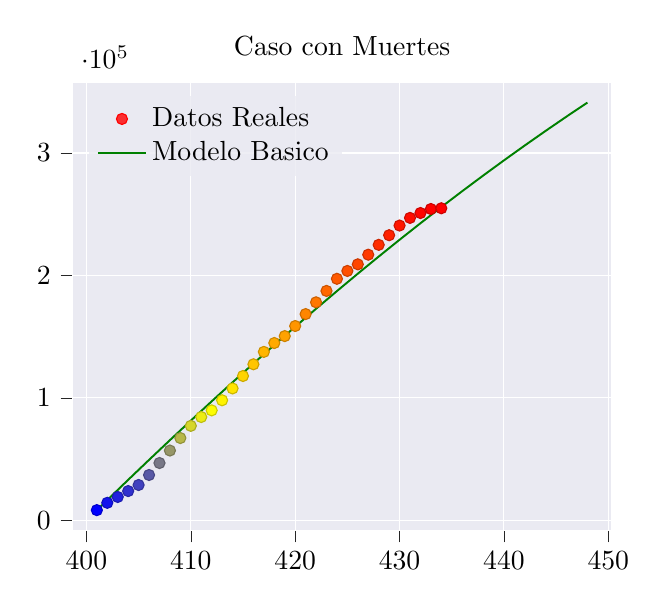
\begin{tikzpicture}

\definecolor{color0}{rgb}{0.917647058823529,0.917647058823529,0.949019607843137}

\begin{axis}[
axis background/.style={fill=color0},
axis line style={white},
legend cell align={left},
legend style={
  fill opacity=0.8,
  draw opacity=1,
  text opacity=1,
  at={(0.03,0.97)},
  anchor=north west,
  draw=none,
  fill=color0
},
tick align=outside,
tick pos=left,
title={Caso con Muertes},
x grid style={white},
xmajorgrids,
xmin=398.65, xmax=450.35,
xtick style={color=white!15!black},
y grid style={white},
ymajorgrids,
ymin=-8319.93961925339, ymax=357868.732004321,
ytick style={color=white!15!black}
]
\addplot [draw=red, fill=red, mark=*, only marks, scatter]
table{%
x  y
401 8325
402 14302
403 19083
404 23893
405 28852
406 37027
407 46810
408 57008
409 67214
410 77152
411 84377
412 89813
413 98062
414 107740
415 117881
416 127446
417 137577
418 144822
419 150471
420 158701
421 168455
422 178076
423 187374
424 197274
425 203682
426 209100
427 216969
428 225001
429 232869
430 240780
431 247016
432 251005
433 254278
434 254890
};
\addlegendentry{Datos Reales}
\addplot [line width=0.7pt, green!50!black]
table {%
401 8325
404 33071.98046875
406 49367.41015625
408 65489.59765625
410 81429.4609375
412 97178.4140625
414 112728.328125
416 128071.6015625
418 143201.125
420 158110.328125
422 172793.09375
424 187243.90625
426 201457.703125
428 215429.96875
430 229156.6875
432 242634.328125
434 255859.875
436 268830.78125
438 281544.96875
440 294000.84375
442 306197.1875
444 318133.28125
446 329808.8125
448 341223.78125
};
\addlegendentry{Modelo Basico}
\end{axis}

\end{tikzpicture}
